\documentclass{article}
\usepackage{tikz}

\begin{document}

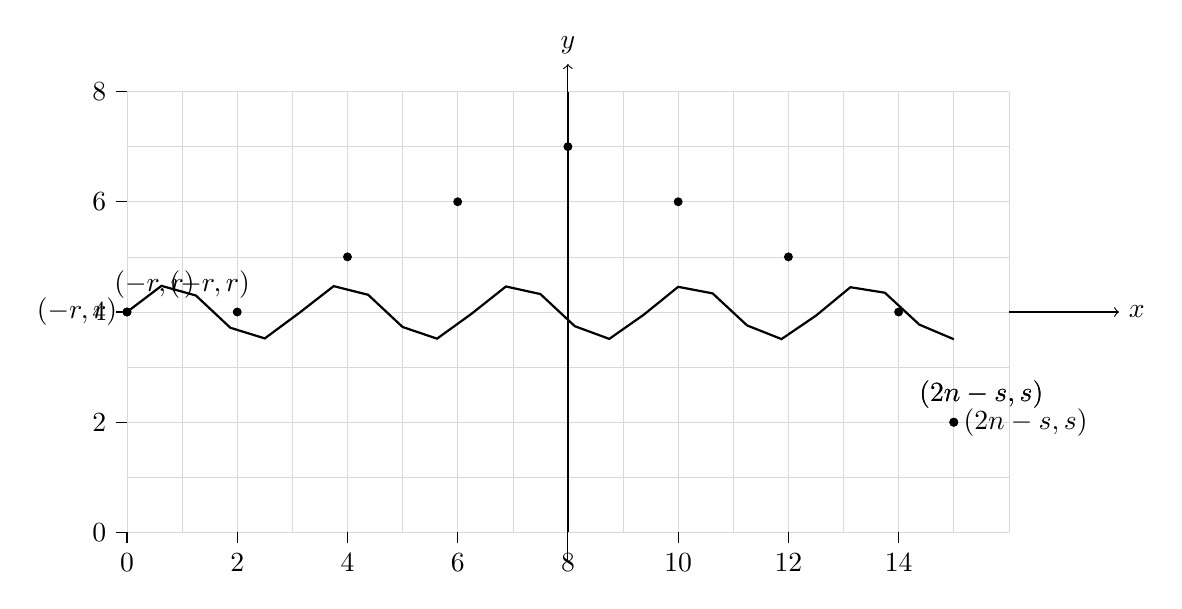
\begin{tikzpicture}[scale=0.7]
    % Draw the grid
    \draw[help lines, color=gray!30] (0,0) grid (16,8);
    
    % Draw the path
    \draw[thick, domain=0:15] plot (\x,{0.5*sin(2*\x r)+4});
    
    % Mark the starting point
    \filldraw[black] (0,4) circle (2pt) node[left] {$( -r , r )$};
    
    % Mark the ending point
    \filldraw[black] (15,2) circle (2pt) node[right] {$( 2n - s , s )$};
    
    % Draw the vertical line
    \draw[thick] (8,0) -- (8,8);
    
    % Label the x-axis
    \draw[->] (16,4) -- (18,4) node[right] {$x$};
    
    % Label the y-axis
    \draw[->] (8,-0.5) -- (8,8.5) node[above] {$y$};
    
    % Label the points on the x-axis
    \foreach \x in {0,2,...,14} {
        \draw (\x,0) -- (\x,-0.2) node[below] {\x};
    }
    
    % Label the points on the y-axis
    \foreach \y in {0,2,...,8} {
        \draw (0,\y) -- (-0.2,\y) node[left] {\y};
    }
    
    % Label the points on the path
    \foreach \x/\y in {0/4,2/4,4/5,6/6,8/7,10/6,12/5,14/4,15/2} {
        \filldraw[black] (\x,\y) circle (2pt);
    }
    
    % Label the points on the path with coordinates
    \node at (0.5,4.5) {$( -r , r )$};
    \node at (15.5,2.5) {$( 2n - s , s )$};
    
    % Label the points on the path with labels
    \node at (1.5,4.5) {$( -r , r )$};
    \node at (15.5,2.5) {$( 2n - s , s )$};
    
\end{tikzpicture}

\caption{A gentle Motzkin path from $(-r,r)$ to $(2n-s,s)$ where $n=13$, $r=4$, and $s=2$.}
\label{fig:motzkin_path}

\end{document}